%                      Code_Saturne version 1.3
%                      ------------------------
%
%     This file is part of the Code_Saturne Kernel, element of the
%     Code_Saturne CFD tool.
%
%     Copyright (C) 1998-2007 EDF S.A., France
%
%     contact: saturne-support@edf.fr
%
%     The Code_Saturne Kernel is free software; you can redistribute it
%     and/or modify it under the terms of the GNU General Public License
%     as published by the Free Software Foundation; either version 2 of
%     the License, or (at your option) any later version.
%
%     The Code_Saturne Kernel is distributed in the hope that it will be
%     useful, but WITHOUT ANY WARRANTY; without even the implied warranty
%     of MERCHANTABILITY or FITNESS FOR A PARTICULAR PURPOSE.  See the
%     GNU General Public License for more details.
%
%     You should have received a copy of the GNU General Public License
%     along with the Code_Saturne Kernel; if not, write to the
%     Free Software Foundation, Inc.,
%     51 Franklin St, Fifth Floor,
%     Boston, MA  02110-1301  USA
%
%-----------------------------------------------------------------------
\section{SOLUTION FOR CASE 4}
This case is similar to case 3, with the following differences:\\
\hspace*{1cm}$\bullet\ $parallel computation on 2 processors\\
\hspace*{1cm}$\bullet\ $head loss\\
\hspace*{1cm}$\bullet\ $calculation of a spatial average\\
\hspace*{1cm}$\bullet\ $dealing with a user results file

The head loss is controlled by the {\itshape uskpdc.F} routine. Some elements
are given in paragraph \ref{prg_case4}. Refer to the example file in the
directory TEST\_CASES for the complete {\itshape uskpdc.F} file.

The calculation of the spatial average is done in the {\itshape usproj.F}
routine. Refer to the example file in the
directory TEST\_CASES for the complete {\itshape usproj.F} file.

The other two changes are controlled in the item
{\itshape Prepare batch analysis}.

To run the calculation on two processors, simply change the number of processors
indicator to 2. The launch script will automatically deal with the rest.

\begin{figure}[h!]
\begin{center}
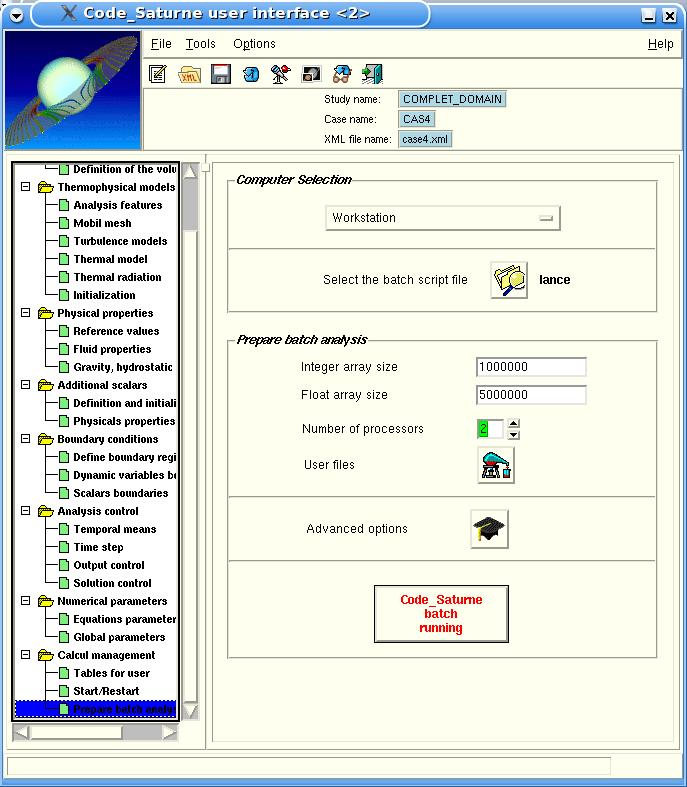
\includegraphics[width=12cm]{\repgraphics/c4_capture01.jpg}
\caption{Number of processors}
\label{fig1_e4}
\end{center}
\end{figure}


\newpage
As seen in paragraph \ref{prg_case4}, the file ``moy.dat'' created by
{\itshape usproj.F} will be written in the temporary execution directory. It
must be identified in the launch script in order to be automatically copied in
the RESU directory (More precisely, a RES\_USERS.xxxxxxxx directory will be
created in the RESU folder, in which the file will be copied).

Click on the icon {\itshape User files} to open the associated dialog window.
Enter the file name ``moy.dat'' in the field {\itshape New results files}
and press the return''Enter'' key on the keyboard. The file name moves to the
list in the above window, so further file names can be added. When finished,
click on {\itshape Validate}.

\begin{figure}[h!]
\begin{center}
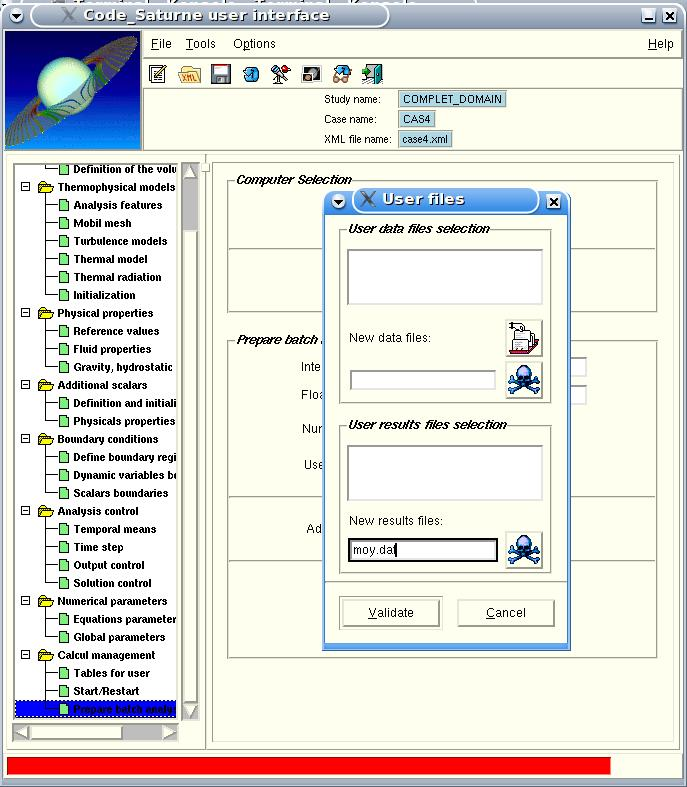
\includegraphics[width=12cm]{\repgraphics/c4_capture02.jpg}
\caption{User results files}
\label{fig2_e4}
\end{center}
\end{figure}


